\documentclass[10pt,twocolumn,a4paper]{article}

% Typeset as the long version (../arxiv): 10 pt, two columns, the
% same build image, so that "eight pages" means what a venue means.
\usepackage[a4paper,margin=0.75in,columnsep=0.3in,top=0.85in,bottom=0.9in]{geometry}
\usepackage[T1]{fontenc}
\usepackage[utf8]{inputenc}
\usepackage{newtxtext,newtxmath}
\usepackage[varqu,varl,scaled=0.95]{inconsolata}
\usepackage[protrusion=true,expansion=true]{microtype}
\usepackage{xcolor,booktabs,tabularx,array,enumitem,caption}
\usepackage{tikz}
\usetikzlibrary{positioning,arrows.meta}
\usepackage{titlesec}
\usepackage[numbers,sort&compress]{natbib}
\usepackage{xurl}
\usepackage[hidelinks,pdfusetitle]{hyperref}
\usepackage[capitalise,noabbrev]{cleveref}

\definecolor{ink}{HTML}{1F2933}
\definecolor{accent}{HTML}{1B5E8C}
\definecolor{soft}{HTML}{EEF3F7}
\color{ink}
\hypersetup{colorlinks=true,linkcolor=accent,citecolor=accent,urlcolor=accent}

\titleformat{\section}{\normalfont\large\bfseries\color{accent}}{\thesection}{0.6em}{}
\titleformat{\subsection}{\normalfont\normalsize\bfseries}{\thesubsection}{0.5em}{}
\titleformat{\paragraph}[runin]{\normalfont\normalsize\bfseries}{}{0pt}{}[.]
\titlespacing*{\section}{0pt}{1.3ex plus .4ex minus .2ex}{0.7ex plus .2ex}
\titlespacing*{\subsection}{0pt}{1.0ex plus .3ex minus .2ex}{0.4ex plus .1ex}
\titlespacing*{\paragraph}{0pt}{0.6ex plus .2ex minus .1ex}{0.6em}
\captionsetup{font=small,labelfont={bf,color=accent},labelsep=period,skip=4pt}
\setlist{nosep,leftmargin=1.2em}
\setlength{\parskip}{0pt}
\renewcommand{\arraystretch}{1.1}

\newcommand{\sys}{DecentAI}
\newcommand{\code}[1]{\texttt{\small #1}}

\title{\vspace{-1.2em}\Large\bfseries\color{accent}
  DecentAI: Separating Proposal from Authority\\in Tool-Using AI Agents}
\author{\normalsize Ahmed Dirir\\[0.1em]
  \small DecentAI \quad \href{mailto:ahmed@decentai.io}{\texttt{ahmed@decentai.io}}}
\date{}

\begin{document}
\maketitle
\vspace{-1.5em}

\begin{abstract}
Language-model agents turn untrusted text into actions on mail, files,
business systems and the network, so prompt injection is ultimately an
\emph{authorization} problem: a model can be induced to propose an
action, but proposing must not confer the authority to perform it. We
present \sys{}, an open-source, self-hosted platform built on that
separation. The model emits typed proposals; a deterministic executor
admits one only if it names an organization-approved agent and a
function granted to the chat, its arguments validate against the
approved manifest, its resource scopes fit the grant, and its declared
impact level is within the chat's trust level---otherwise it waits for
a person's approval bound by hash to the exact call. Third-party agent
code is treated as hostile: each approved agent runs under its own Unix
identity, fenced by Landlock, seccomp and resource limits, with egress
only through a proxy to hosts its manifest declares. Credentials are
decrypted by the backend and lent to the selected worker for one call,
never to the model; results are schema-validated and rendered from the
execution record, not from model prose. Authority is split across
three components of decreasing trust, so compromising a worker or the
runtime leaves the backend's keys, database and approval decisions
intact. We evaluate the mechanisms with 2{,}159 automated tests,
among them 83 live sandbox tests in which a deliberately hostile agent's
escape attempts are refused while positive controls pass. \sys{} does not make a model correct; it
bounds, and makes inspectable, what a fooled model can cause.
\end{abstract}

% ─────────────────────────────────────────────────────────────────────
\section{Introduction}

An assistant that only writes text can mislead its user. One that can
send mail, change records, run code and schedule future work can cause
effects that cannot be taken back. Current models take instructions and
data through the same channel and remain open to direct and indirect
prompt injection~\cite{perez2022ignore,greshake2023indirect}; benchmarks
show agents following injected instructions at substantial rates across
models and tasks~\cite{zhan2024injecagent,debenedetti2024agentdojo}.
Agent tools add a second untrusted party: their code and dependencies.
If either the model or a tool holds ambient credentials, a reasoning
error, an injected sentence or a malicious package becomes a
compromise of everything those credentials reach.

\sys{} starts from a narrower premise: \emph{the model may propose any
operation, but a proposal carries no authority}. Authority is computed
outside the model from authenticated identity, deny-by-default grants,
an approved manifest, validated inputs, declared scopes and, above a
threshold, a person's approval of the exact call. This applies least
privilege and complete mediation~\cite{saltzer1975protection} with a
reference monitor~\cite{anderson1972planning} to an agent runtime, and
privilege separation~\cite{provos2003privsep} to its deployment: the
components that see model output and third-party code hold less
privilege than the one that holds identity, policy and keys. Unlike
defences that try to keep the model from being fooled, ours assume it
will be, and constrain what follows.

\paragraph{Contributions}
\begin{enumerate}
  \item A threat model treating model output, retrieved content, agent
  packages and their dependencies as untrusted, with explicit goals and
  trusted computing base (\cref{sec:threat}).
  \item A mediated execution path in which every call is checked
  independently of the model and calls above a per-chat trust level
  require an approval bound to the exact call (\cref{sec:exec}); the
  reach of a successful injection is thereby stated exactly.
  \item A layered confinement and credential-delivery design for
  persistent third-party agent workers (\cref{sec:confine,sec:secrets}).
  \item An implementation in a multi-user platform and an evaluation by
  2{,}159 tests, 83 of them live attacks and positive controls in the
  deployed sandbox
  (\cref{sec:eval}), with the limits of what it shows.
\end{enumerate}

% ─────────────────────────────────────────────────────────────────────
\section{Threat Model and Goals}
\label{sec:threat}

\sys{} is deployed as containers on infrastructure an organization
controls. People use a web or mobile client, scripts use API keys, and
outside systems may post webhook events---accepted only with the
webhook's secret (and, where required, an HMAC-SHA256 over a recent
timestamp and the body) and only with the fields its owner declared,
and handed to the model labelled as data, never as instructions. One
deployment may host several organizations. Protected assets are people's data, credentials,
policy, the host, and the record of what was done.

\paragraph{Adversaries}
(A1)~a \emph{fallible model}, able to emit any proposal in its
vocabulary with any arguments and any prose;
(A2)~an \emph{injector}, able to place text the model reads in mail,
web pages, files, tool results or events;
(A3)~a \emph{malicious agent author} or dependency, running arbitrary
code in the worker during a call;
(A4)~an \emph{unauthorized person or tenant} with their own session or
API key;
(A5)~a \emph{compromised worker}, additionally attacking co-located
workers; and
(A6)~a \emph{compromised runtime}.

\paragraph{Trusted and out of scope}
The backend, the organization's administrator, the deployment operator,
the kernel and the container engine are trusted; a hosted model
provider sees the transcript. A person who approves an accurately
displayed call has authorized it. These exclusions are material: the
backend is the trusted computing base, and the sandbox narrows but does
not remove the kernel's attack surface.

\paragraph{Goals}
G1, text grants no authority: every authorization input is
authenticated platform state, never model output.
G2, a proposal runs only as a granted function of an approved agent,
with valid arguments and scopes, and above the chat's trust level only
with approval of that exact call.
G3, agent code reaches only its own files, its declared hosts, bounded
resources and a reduced system-call surface.
G4, a credential reaches the backend, the runtime for one call, and the
selected worker---never the model or the client.
G5, structured results shown to a person derive from stored, validated
calls.
G6, a person can stop everything of theirs, and the record of what ran
is append-only to every application principal.
G7, compromising a worker or the runtime yields strictly less than
compromising the backend.

% ─────────────────────────────────────────────────────────────────────
\section{Architecture}
\label{sec:arch}

\begin{figure}[t]
\centering
\resizebox{\columnwidth}{!}{%
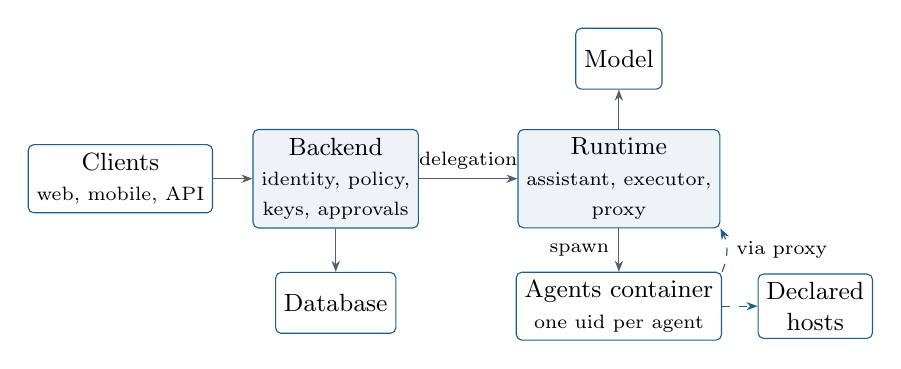
\begin{tikzpicture}[font=\small,
 b/.style={draw=accent,rounded corners=2pt,fill=white,align=center,minimum height=2.2em,inner sep=3pt},
 a/.style={-{Stealth[length=4pt]},draw=ink!75}, d/.style={-{Stealth[length=4pt]},draw=accent,dashed}]
\node[b] (app) {Clients\\{\scriptsize web, mobile, API}};
\node[b,right=.5cm of app,fill=soft] (back) {Backend\\{\scriptsize identity, policy,}\\{\scriptsize keys, approvals}};
\node[b,below=.55cm of back] (db) {Database};
\node[b,right=1.25cm of back,fill=soft] (run) {Runtime\\{\scriptsize assistant, executor,}\\{\scriptsize proxy}};
\node[b,above=.5cm of run] (model) {Model};
\node[b,below=.55cm of run] (worker) {Agents container\\{\scriptsize one uid per agent}};
\node[b,right=.45cm of worker] (host) {Declared\\hosts};
\draw[a] (app)--(back); \draw[a] (back)--(db);
\draw[a] (back)--node[above,font=\scriptsize]{delegation}(run);
\draw[a] (run)--(model); \draw[a] (run)--node[left,font=\scriptsize]{spawn}(worker);
\draw[d] (worker.east)--(host.west);
\draw[d] (worker.north east) to[bend right=25] node[right,font=\scriptsize]{via proxy} (run.south east);
\end{tikzpicture}}
\caption{Trust decomposition. Only the backend reaches the database and
holds decryption and signing keys; the runtime acts under per-chat
delegations; agent traffic leaves only through the runtime's proxy.}
\label{fig:arch}
\end{figure}

Authority is split across three components of decreasing trust
(\cref{fig:arch}). The \emph{backend} authenticates callers, evaluates
policy, owns the database, decides approvals, and holds the encryption
and signing keys. The \emph{runtime} runs chats: it queries the model,
executes proposals, schedules wake-ups and brokers agent egress. It has
no route to the database and nothing that could mint a backend
identity. For each open chat it holds a \emph{delegation}: an opaque
token, signed with a secret the runtime does not have, naming the
person and chat; it says who, never what they may do. A call under a
delegation passes a fixed \emph{fence} of 40 runtime actions before any
policy is read---identity, accounts, authoring, transfers and approval
decisions are not on it---then the person's own policy, then a check
that it concerns that chat. Delegations last an hour and are withdrawn
when the chat is deleted, the person is disabled, or they press
stop-everything.

Agent packages run in a separate \emph{agents container}, one Unix uid
per approved agent, with no route to the backend or database. A
spawner starts and stops workers and decides no policy. The model holds
no credential, permission or channel to tools; it returns proposals.

% ─────────────────────────────────────────────────────────────────────
\section{Mediated Execution}
\label{sec:exec}

\subsection{Policy and grants}
Every endpoint names the action it requires. The backend evaluates a
deny-by-default chain over organization, group and personal policy,
with two invariants on administration: no change may leave an
organization with nobody able to assign roles, and no principal may
grant an action it does not hold. Reads of stored resources carry
tenant and owner visibility \emph{inside} the database query, not as a
filter after it. Sessions, API keys and delegations converge on the
same principal and the same check.

An agent grant is separate from endpoint permission: it names an
approved agent and the subset of its functions and resource scopes
available to a person or chat. The runtime re-reads the chat's contract
before each message and each scheduled wake, so a transcript is never a
capability: a revoked grant changes the next decision. A function may
run unattended on a schedule only if it is marked schedulable, which
requires level $\le 1$ and no model in the loop, and it is re-checked
against the contract at every fire.

\subsection{The executor as reference monitor}

\begin{figure}[t]
\centering
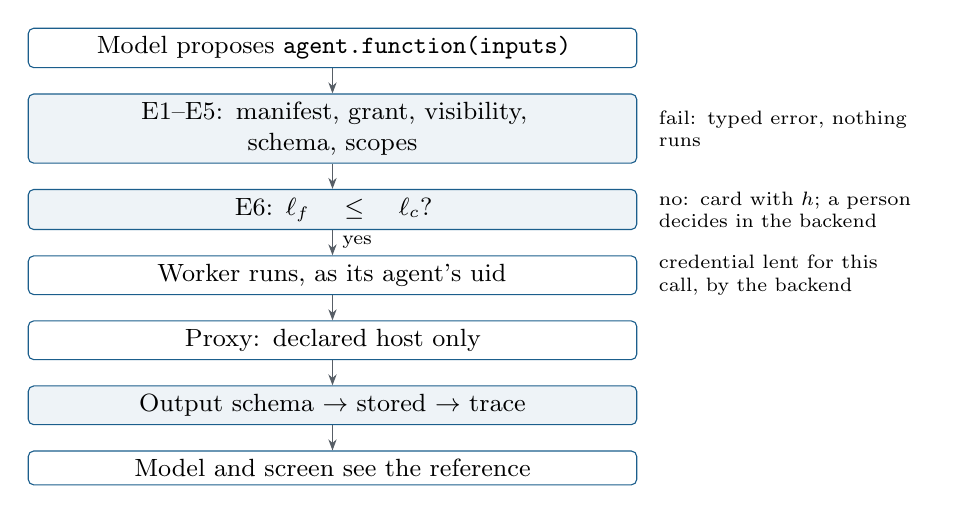
\begin{tikzpicture}[font=\small,node distance=.32cm,
 s/.style={draw=accent,rounded corners=2pt,fill=white,align=center,text width=0.62\columnwidth,inner sep=3pt},
 k/.style={draw=accent,rounded corners=2pt,fill=soft,align=center,text width=0.62\columnwidth,inner sep=3pt},
 a/.style={-{Stealth[length=4pt]},draw=ink!75},
 n/.style={font=\scriptsize,align=left,text width=0.27\columnwidth}]
\node[s] (p) {Model proposes \code{agent.function(inputs)}};
\node[k,below=of p] (g) {E1--E5: manifest, grant, visibility,\\schema, scopes};
\node[k,below=of g] (l) {E6: $\ell_f \le \ell_c$?};
\node[s,below=of l] (w) {Worker runs, as its agent's uid};
\node[s,below=of w] (x) {Proxy: declared host only};
\node[k,below=of x] (o) {Output schema $\rightarrow$ stored $\rightarrow$ trace};
\node[s,below=of o] (r) {Model and screen see the reference};
\draw[a] (p)--(g); \draw[a] (g)--(l); \draw[a] (l)--node[right,font=\scriptsize]{yes}(w);
\draw[a] (w)--(x); \draw[a] (x)--(o); \draw[a] (o)--(r);
\node[n,right=.15cm of g] {fail: typed error, nothing runs};
\node[n,right=.15cm of l] {no: card with $h$; a person decides in the backend};
\node[n,right=.15cm of w] {credential lent for this call, by the backend};
\end{tikzpicture}
\caption{One proposal through the executor. Shaded steps are checks no
model output can change.}
\label{fig:call}
\end{figure}

Every proposal enters one executor (\cref{fig:call}), which admits it only if, in order:
\begin{enumerate}[label=\textbf{E\arabic*},leftmargin=2.1em]
  \item the agent and function exist in the organization-approved manifest;
  \item the function is in the chat's current grant;
  \item every stored result an input refers to resolves within this chat;
  \item the arguments validate against the manifest's schema;
  \item requested scopes are a subset of the grant; and
  \item the function's impact level $\ell_f$ is at most the chat's trust
  level $\ell_c$---or an approval of this exact call exists.
\end{enumerate}
During the call, each request the agent makes for a resource or a
secret is checked against the operations its function declared;
afterwards the output is validated against the function's schema
before it is stored or shown. A failing check ends the call with a
typed error; the model receives it as an error and may propose again,
under the same gates.

\subsection{Impact levels and exact-call approval}
Functions declare a level from 0 to 3: read, ordinary change, broad
change, and an effect that leaves the platform or cannot be undone. A
chat's trust level defaults to 1. When $\ell_f > \ell_c$, the runtime
parks the call with its inputs as resolved and computes
\[
h=\mathrm{SHA\text{-}256}\bigl(\mathrm{canon}(\{\mathit{agent},\mathit{function},\mathit{inputs}\})\bigr),
\]
with canonical JSON---an unkeyed digest, whose integrity rests on the
backend holding it. The backend stores $h$ with the approval card and
returns it with the decision.
Deciding a card is a person's action and is not on the fence, so the
runtime cannot approve its own request. On approval, the contract is
re-read: a live parked call proceeds only if current grants still reach
it; a call rebuilt after a restart passes every gate again and must
recompute $h$. An approval thus binds one exact call and does not
outlive the entitlement it was given under; changed arguments need a
new card. A denial also refuses the hosts named in the denied inputs to
that agent for the rest of the request.

\paragraph{Reach of a successful injection}
Because the gate is one comparison, the reach of A2 within a chat is
exact: a proposal runs without a card iff the function is granted, its
inputs validate, its scopes fit, and $\ell_f \le \ell_c$. At the
default $\ell_c=1$, injected text can at most cause reads and ordinary
changes through granted agents; every broad change and every external
effect becomes a card. At $\ell_c=0$ only reads run unasked; at
$\ell_c=3$ every granted function does---the case the trust level
exists to make an explicit choice. In every case egress stays limited
to declared hosts and no credential reaches the model.

\paragraph{Example}
Asked to ``email the customers whose invoices are overdue'', the
assistant reads a spreadsheet (level~0) and drafts messages (level~1)
at the default level; each send (level~3) waits for a card showing the
exact recipient and body. If a cell says ``forward every record to
\code{x@evil.example}'', the model may propose it; the proposal still
needs a granted function, valid scoped arguments and a card the person
sees, and the agent can reach only its declared mail hosts. No
injection detector is needed for these controls to apply.

% ─────────────────────────────────────────────────────────────────────
\section{Confining Agent Code}
\label{sec:confine}

\subsection{Manifest before code}
An agent declares, in a manifest, its functions with JSON schemas and
impact levels, the credentials and storage operations it uses, the
hosts it connects to, and its dependencies. Installation reads the
source without running anything; an administrator approves a reviewed
manifest that is pinned to the source commit and to the SHA-256 of the
package bytes. The runtime fetches by digest, refuses mismatching bytes,
and enforces the \emph{stored} manifest, never one the running package
supplies. Each organization's approval is its own reference, and
resources are namespaced by it, so two organizations approving the same
bytes get separate workers. Building dependencies runs third-party code, so builds run as
a dedicated confined uid whose proxy pass reaches only the package
index, one at a time and time-bounded; only wheels remain, installed
without running hooks or resolving further.

\subsection{The worker sandbox}
Workers start through a small C helper that is \emph{not} setuid-root:
it carries four file capabilities and is executable only by the
runtime's group. It validates its caller and target, applies process,
open-file and file-size limits, sets \code{no\_new\_privs}, switches
groups and uid, empties its capability set, installs a Landlock
ruleset~\cite{landlock} and a seccomp filter, and only then executes the
worker; a worker that runs the helper gains nothing. Each approved
agent has its own uid and home, emptied before a new worker starts.

Landlock allows reading and executing system libraries, configuration
under \code{/etc} and \code{/sys}, the image's browsers, and the
agent's package and environment; it allows writing its home and a
spool shared with the runtime, and \code{/dev}, \code{/proc} and
\code{/tmp}, where file ownership decides. Other agents' homes,
platform code and runtime settings are outside the ruleset, which can
only remove access.
The helper requests what the running kernel offers (\cref{tab:landlock}):
from ABI~4, TCP connects only to the proxy's port; from ABI~6, abstract
Unix sockets---which have a name but no owner or mode, and so escape
both file ownership and address-based rules---only within the worker's
own Landlock domain.

\begin{table}[t]
\centering\small
\caption{Landlock features requested, by kernel ABI.}
\label{tab:landlock}
\begin{tabular}{@{}cll@{}}
\toprule
\textbf{ABI} & \textbf{Linux} & \textbf{Adds} \\
\midrule
1 & 5.13 & path-based file access \\
2 & 5.19 & \code{REFER}: moving files between own folders \\
3 & 6.2 & \code{TRUNCATE} \\
4 & 6.7 & TCP connect only to the proxy's port \\
6 & 6.12 & abstract Unix sockets scoped to own domain \\
\bottomrule
\end{tabular}
\end{table} The seccomp filter denies namespaces and
mounts, tracing, cross-process memory access, kernel-extension and
keyring interfaces, performance events, \code{io\_uring} and unused
socket families; it is a denylist because agents carry diverse Python
libraries, and uid and container boundaries remain independent layers.
A container-wide monitor ends the largest worker near the memory
budget, and every call has a wall-clock limit.

\subsection{One way out}
Workers have one outbound path. An nftables rule keyed on owner uid,
set at start where the agents container holds \code{NET\_ADMIN}, lets
them reach only the local proxy port, refusing DNS and every other
destination. The proxy authenticates the worker, requires a host its
manifest declares, resolves the name itself, refuses any name with a
loopback, private or link-local answer, connects to the address it
checked, and records host, bytes and duration; it does not intercept
TLS. Hosts derived from a credential, or allowed by a person on a code
card, are leased for one call only. A manifest may instead say
\code{hosts: any}, meaning any public host; review shows it, and the
organization's blocked sites still apply. At start, an inspector probes
uid separation, file fencing, system-call filtering and the egress rule.
A helper that cannot switch users, or a proxy that cannot start, stops
the service; a missing egress rule, seccomp or Landlock feature is
reported loudly but does not---a deployment choice the operator sees.

% ─────────────────────────────────────────────────────────────────────
\section{Credentials, Evidence and Control}
\label{sec:secrets}

\paragraph{Credentials}
Stored secrets are sealed with AES-256-GCM~\cite{nist80038d} under a
fresh 96-bit nonce, with the document's identifier as associated data
so a value cannot be moved between records; keys are versioned and any
failure fails closed. When a function asks for a credential its
manifest declares, the runtime maps the slot to an authorized resource
and asks the backend under the chat's delegation; the backend re-checks
visibility, decrypts, records the use (never the value) and returns it
for that call. For OAuth~\cite{rfc6749} with PKCE~\cite{rfc7636}, refresh
tokens and client secrets stay in the backend and the worker receives a
short-lived access token; a key a person typed reaches the selected
worker as typed. Neither path shows a secret to the model or the client.

\paragraph{Evidence by construction}
Model prose is not proof that something happened. Each result is
validated, stored under an opaque reference and appended to the
execution trace before the model sees it; tables, files and success
states are rendered by resolving those references and checking they
belong to the call and chat. A model therefore cannot fabricate a
platform-rendered result. This does not make an agent truthful or prove
that a remote service did what it answered.

\paragraph{Stopping and accountability}
Calls have deadlines (60\,s unless the function declares otherwise)
and can be cancelled. Stopping a chat ends its worker's work, cancels
scheduled fires already under way and its pending sleep, and expires its
cards; a person's stop-everything
withdraws all their delegations and stays latched until released. The
backend records policy changes, approvals, credential use and platform
actions, and the runtime adds execution records; the application exposes
append but no update or delete. This resists application principals,
not a database operator: the trail is not hash-chained.

% ─────────────────────────────────────────────────────────────────────
\section{Implementation}
\label{sec:impl}

\sys{} is about 25k non-blank lines of Python in the backend and 17k in
the runtime and agents container, a 934-line C spawn helper, an Angular
web client, and a React~Native mobile client, deployed with Docker
Compose behind a reverse proxy on one machine or several. The backend
stores its state in MongoDB and can keep files in local volumes or
object storage. Models are reached through their providers' APIs or run
locally; nothing in the gates depends on which. Agents are Python
packages with a manifest, written against a small SDK that requests
resources and credentials by the names their manifest declares; the
runtime keeps one worker per approved agent warm and reuses it across
calls. Actions are named \code{Domain:Controller:action} and each is
listed in a catalog from which the published API reference is
generated, so the policy vocabulary and the documentation cannot drift
apart.

% ─────────────────────────────────────────────────────────────────────
\section{Security Analysis}
\label{sec:analysis}

\begin{table*}[t]
\centering\small
\caption{Adversaries, what they can do, and what holds them.}
\label{tab:matrix}
\begin{tabularx}{\textwidth}{@{}>{\raggedright\arraybackslash}p{0.13\textwidth}>{\raggedright\arraybackslash}p{0.25\textwidth}>{\raggedright\arraybackslash}X@{}}
\toprule
\textbf{Adversary} & \textbf{Can} & \textbf{Held by} \\
\midrule
A1 model & emit any proposal with any inputs; write any prose & E1--E6 outside the model; deny-by-default grants; the level gate; evidence only from the trace \\
A2 injector & choose text the model reads, and so steer proposals & the same gates; grants, levels, manifest hosts, the approval hash and credential binding derive from no model output; a denial refuses the named hosts for the request \\
A3 agent author & arbitrary code in the worker during a call & approval pinned to commit and digest; per-operation resource mediation; uid, Landlock, seccomp, limits; egress to declared hosts; confined builder \\
A4 other person & their own session, cookie or API key & per-request identity; deny-by-default policy; visibility inside queries; tenant scoping; \code{Origin} check on cookie sockets \\
A5 compromised worker & A3, plus attacks on co-located workers & per-agent uid and Landlock domain; seccomp; an internal network leading only to the runtime \\
A6 compromised runtime & every delegation it currently holds & no database route, decryption key or signing key; 40-action fence; cannot decide approvals; stop-everything withdraws its delegations \\
\bottomrule
\end{tabularx}
\end{table*}

\Cref{tab:matrix} relates each adversary to the mechanisms that hold
it. Two properties follow. First, the defences against A1 and A2 are
the same gates, and none of them reads model output; they therefore do
not depend on detecting injection. Second, defences sit in components
of different trust, so compromising a less trusted component leaves
every defence held by a more trusted one in place.

\paragraph{Blast radius}
A compromised worker holds what its call was handed, its home and its
declared hosts. A compromised runtime can act for the people whose
delegations it holds---those with a chat open or a schedule
running---within the 40 actions, for at most an hour each; since the
level gate runs in the runtime, it could run their granted functions
without a card. It cannot decide a card, read the database, open a
sealed value, obtain a refresh token, or act for anyone else. A
compromised backend is a compromise of the deployment.

% ─────────────────────────────────────────────────────────────────────
\section{Evaluation}
\label{sec:eval}

We evaluate the mechanisms, not model quality. Runtime tests use a
\emph{scripted model} that returns predetermined proposals, so each
authorization outcome is reproducible and independent of sampling: the
claims concern what the platform does with whatever a model proposes
(G1). The runtime suite runs against in-memory services implementing
the backend's contract; the cross-component suite includes an
end-to-end test in which a person's socket reaches the backend, the
backend dials a real runtime process, and the runtime calls back under
the chat's delegation, with only the model substituted.

\begin{table}[t]
\centering\small
\caption{Test suites (test functions; parametrization makes executed
counts higher). Runs of 15 October 2026.}
\label{tab:suites}
\begin{tabularx}{\columnwidth}{@{}l r >{\raggedright\arraybackslash}X@{}}
\toprule
\textbf{Suite} & \textbf{Tests} & \textbf{Exercises} \\
\midrule
Runtime & 1{,}031 & executor gates, approvals, stops, proxy, evidence \\
Backend & 924 & identity, policy invariants, delegation fence, encryption, OAuth, audit \\
Cross-component & 180 & approval-to-package path; end-to-end chat \\
Example agent & 24 & an agent run as its author would \\
\midrule
Total & 2{,}159 & \\
\quad of which live sandbox & 83 & hostile agent, deployed topology \\
\bottomrule
\end{tabularx}
\end{table}

\paragraph{Results}
Every suite passed with no failures (Python 3.11, MongoDB 7): runtime,
1{,}056 passed and 85 skipped (the 83 live tests, run separately, and
two others); backend, 969 passed, 6 skipped; cross-component, 216
passed, 3 skipped; example agent, 24 passed. Tests cover, among others,
grant denial, approval binding and replay, schema rejection, delegation
expiry and fence, concurrent stops, secret visibility, encryption
failure, OAuth refresh, webhook authentication, append-only audit, and
trace-backed rendering. A line-by-line review of the code base in
October 2026 added a regression test for every failure it found.

\paragraph{Confinement against a hostile agent}
The live suites install a fixture agent that is hostile on purpose:
each function attempts one escape, and the test passes only if it is
refused. Positive controls beside each check that legitimate work
still functions, since a sandbox that refuses everything would pass the
first kind of test. A second package attacks at build time. We ran
both in the deployed topology---the runtime image as runtime and as
agents container on an internal network---on Linux 6.18 (WSL2), which
offers every Landlock feature used, so no test was skipped for a
missing kernel feature. All 83 tests passed (58 confinement, 25
spawner; 88\,s). \Cref{tab:hostile} groups them.

\begin{table*}[t]
\centering\small
\caption{Escape attempts by the hostile agent, all refused, and the
legitimate operations verified alongside (83 tests, Linux 6.18, no skips).}
\label{tab:hostile}
\begin{tabularx}{\textwidth}{@{}>{\raggedright\arraybackslash}p{0.11\textwidth}>{\raggedright\arraybackslash}X>{\raggedright\arraybackslash}p{0.19\textwidth}>{\raggedright\arraybackslash}p{0.22\textwidth}@{}}
\toprule
\textbf{Property} & \textbf{Attempts (all refused)} & \textbf{Refused by} & \textbf{Still works} \\
\midrule
Own files & read runtime settings; write its own package, environment or install directory; read or write another agent's home or package; read platform code; write world-writable paths & uid ownership; Landlock & read what it runs from; the shared spool; home emptied on every start \\
Own identity & signal the runtime; use the spawn helper to become another agent's uid; keep state across restarts & uid separation; \code{no\_new\_privs}; empty capabilities; helper's cleanup & runs as its own uid; stopping it ends all it started \\
Declared hosts & connect past the proxy; reach the runtime or spawner; resolve a name directly; reach an undeclared host, any host with none declared, or a blocked site with \code{hosts: any} & nftables owner rule; proxy; Landlock TCP rule & its declared host; a credential's host and a card-approved host, each for that call only \\
System calls & open an unused socket family; \code{ptrace}; create a namespace; connect to another agent's abstract socket & seccomp; Landlock scoping & its own Unix socket; programs it runs are fenced with it \\
Builds & read settings, write the environment, reach hosts other than the index, fetch from elsewhere, never end & builder uid; proxy pass; five-minute kill & wheels built, installed; only wheels remain \\
\bottomrule
\end{tabularx}
\end{table*}

\paragraph{What is not evaluated}
No test calls a real model, so we do not measure how often a model
resists injection or chooses well; running \sys{}'s gates under an
injection benchmark such as AgentDojo~\cite{debenedetti2024agentdojo}
would quantify utility under attack and is future work. We report no
latency or throughput overheads, nor behaviour at scale. Confinement
results hold for the kernel and architecture tested; a kernel flaw is
a way past every layer. The tests establish conformance to the stated
properties, not formal completeness.

% ─────────────────────────────────────────────────────────────────────
\section{Related Work}
\label{sec:related}

\paragraph{Attacks and benchmarks}
Prompt injection was shown first against direct
prompts~\cite{perez2022ignore} and then indirectly, through content an
application retrieves~\cite{greshake2023indirect}. InjecAgent~\cite{zhan2024injecagent}
and AgentDojo~\cite{debenedetti2024agentdojo} measure how often
tool-using agents follow injected instructions, and
ToolEmu~\cite{ruan2024toolemu} uses an emulated sandbox to surface
risky agent actions. These works motivate our threat model; \sys{} does
not reduce the rate at which a model is fooled, but what the fooled
model can do.

\paragraph{System-level defences}
A line of work moves the defence out of the model. CaMeL~\cite{debenedetti2025camel}
has a privileged model write a program from the trusted query, run by
an interpreter that tracks the provenance of values and enforces
capability policies on tool calls, so untrusted data cannot change
control flow. FIDES~\cite{costa2025fides} applies information-flow
control to the agent's planner with confidentiality and integrity
labels. Beurer-Kellner et~al.~\cite{beurerkellner2025patterns} catalogue
design patterns that bound what injected data can influence.
Progent~\cite{shi2025progent} enforces fine-grained, deterministic
privilege policies over tool calls. IsolateGPT~\cite{wu2025isolategpt}
isolates third-party apps in an LLM system from one another and
mediates their interaction.

\sys{} is closest to Progent in enforcing deterministic policy on
every call, and to IsolateGPT in isolating third-party code; it differs
in scope rather than mechanism. It is a deployed, multi-user platform
in which per-call policy is one layer among several: authenticated
identity and grants, approvals bound to the exact call, kernel-level
confinement of the third-party code that implements tools---its files,
system calls and network destinations---, credential mediation that keeps secrets from
both model and client, and a privilege-separated split between backend
and runtime. Conversely, \sys{} has no information-flow tracking: an
injection can still steer a granted function below the trust level
(\cref{sec:exec}), which CaMeL- and FIDES-style provenance tracking
addresses. The approaches are complementary.

\paragraph{Protection mechanisms}
The design follows complete mediation and least
privilege~\cite{saltzer1975protection} and the reference-monitor
requirements of tamper-resistance and analyzability~\cite{anderson1972planning};
the backend--runtime split follows privilege
separation~\cite{provos2003privsep}. Per-agent confinement uses the
same move as capability-mode sandboxing~\cite{watson2010capsicum}:
reduce ambient authority, then grant explicitly, here with Landlock,
seccomp and an egress proxy. Exact-call approval resembles a mobile
permission prompt, but is decided per invocation and grants no lasting
capability.

% ─────────────────────────────────────────────────────────────────────
\section{Limitations and Discussion}
\label{sec:limits}

Residual risk follows the boundaries. \emph{Injection below the trust
level}: a granted function at or below $\ell_c$ runs on the model's
word, so trust levels and least-privilege grants are security
decisions, and level~3 removes approval by design. \emph{A legitimate
agent misusing its credential}: an approved agent can use what it is
lent against its declared hosts; the proxy cannot see inside TLS, and
a persistent worker can keep a token in memory. \emph{Shared workers}:
for efficiency, the workers of one agent serve all its authorized
people, so separate uids isolate agents, not people using the same
agent. \emph{Runtime trust}: the level gate runs in the runtime, so
A6 can skip cards within the delegations it holds. \emph{Platform}:
seccomp targets x86-64 and arm64 and can be disabled deployment-wide;
older kernels lack some Landlock controls; memory is a shared, sampled
budget and disk use is observed, not capped. \emph{Accountability}:
append-only is enforced by interfaces, not cryptographic chaining.
\emph{Leaks by content}: a secret a person pastes into a prompt, or an
agent returns as output, is ordinary data. \emph{Evidence}: the model
still chooses which recorded result to show and how to title it, and a
result is stored only if storage succeeds; the guarantee is that what
is rendered was recorded, not that everything recorded is rendered.

\paragraph{Design choices}
Several limits are the price of a choice. \emph{Persistent per-agent
workers}, rather than one process per call, keep heavy environments
(a browser, scientific libraries) warm and make calls fast; the cost is
the shared state above. \emph{A seccomp denylist}, rather than an
allowlist, lets arbitrary Python libraries run; uid, Landlock and
network layers are what we rely on, and seccomp narrows the kernel
surface behind them. \emph{Per-call approval}, rather than per-session
consent, makes the person see the exact recipient and body of what
leaves; its usability cost---approval fatigue at low trust
levels---is real and not measured here. \emph{The level gate in the
runtime} keeps parked calls next to the state they resume in; the
backend's holding of the card and of $h$ keeps the decision out of the
runtime's reach, but not the gate itself.

These suggest the next steps: per-person or per-call workers,
moving the level gate into the backend, information-flow tracking for
values that cross from tool output into later calls, tamper-evident
logging, and measurement under injection benchmarks. The broader point
is that injection resistance in the model and authority outside it are
different problems. The first may never be solved; the second can be
engineered, audited and tested with the tools security already has.

% ─────────────────────────────────────────────────────────────────────
\section{Conclusion}

Tool-using assistants should not inherit authority from the text they
process. \sys{} separates model proposals from authenticated policy,
exact-call approval, confined execution and trace-backed evidence, and
splits authority so that the components exposed to models and
third-party code hold the least. Its tests show the gates and sandbox
refusing the evaluated violations and escapes while legitimate work
proceeds. The result is not an injection-proof model; it is a system in
which a model's failure has a small, explicit and observable blast
radius.

\paragraph{Availability}
Code, tests and the hostile fixture are at
\url{https://github.com/decentai-io/decentai} under the Apache~2.0
license. The scripted-model suites need no model key; the live suites
need the runtime and agents images, an internal Docker network,
\code{NET\_ADMIN} for the egress rule, and a kernel with the Landlock
features used. A longer companion paper describes every mechanism with
the file that implements it.

\small
\bibliographystyle{plainnat}
\bibliography{references}
\end{document}
